\documentclass{utue} %utue.cls required for Uni Tuebingen corporate design


\def \myTitle {Tensorflow Implementation of Deep Photo Style Transfer} %TODO
\def \myAuthor {Paul Sanzenbacher, Sebastian Penhou\"{e}t}
\def \myUniversity {University of Tübingen}
\def \myClass {Computer Graphics Practical Course}
\def \myDepartment {Department of Computer Science}
\def \myKeywords {style transfer, tensorflow}

% Values for title generation
\title{\myTitle}
\author{\myAuthor}
\date{\today}

% Subtitle is optional. It represents what kind of work you did.
\subtitle{Winter Term 2017}

\usepackage{preamble}

\begin{document}

% You can place a teaser as follows. (Otherwise, just uncomment the following part)
%\teaser{
    %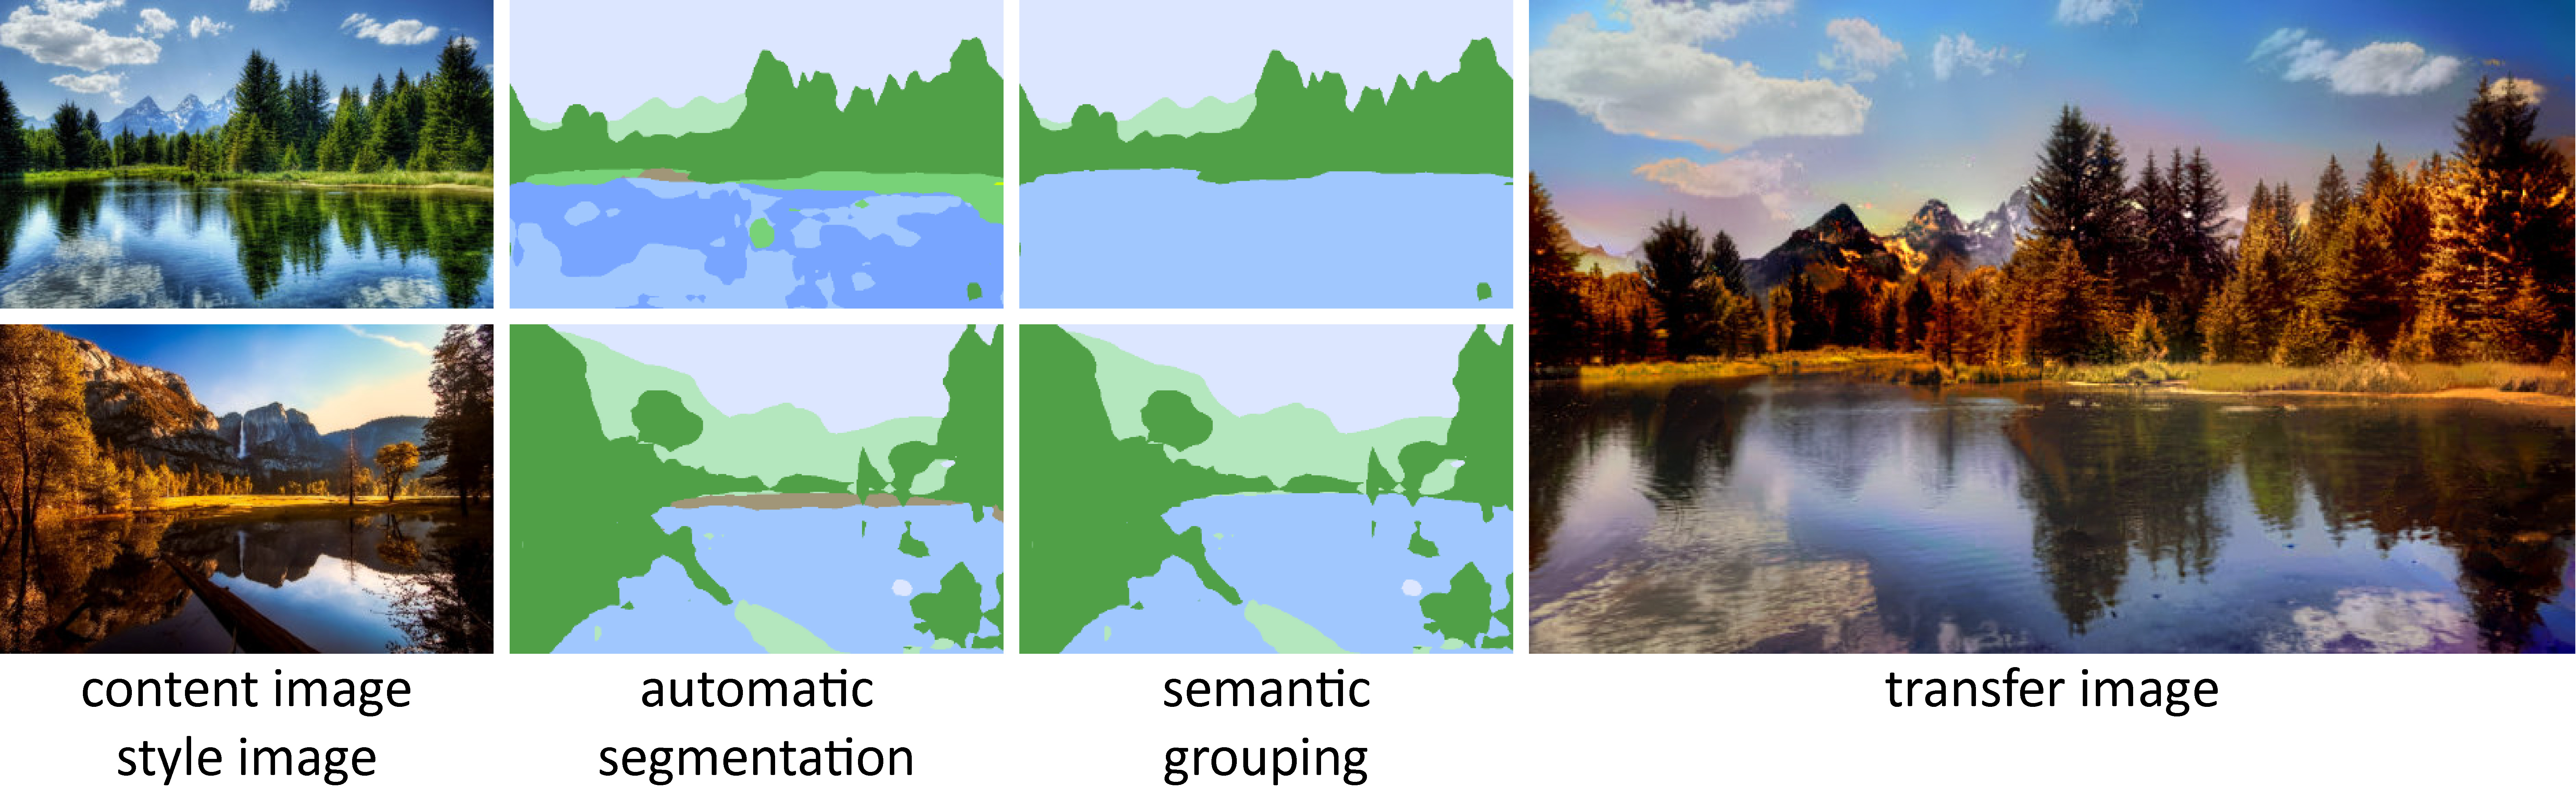
\includegraphics[width=\textwidth]{images/teaser.jpg}
    %\caption{\label{fig:teaser}You can place a teaser here.}
%}

% Creates title of document and additional title page.
\maketitle

\subfile{doc_abstract}

%--------------------------------------------------

\subfile{doc_introduction}

\subfile{doc_style_transfer}

%--------------------------------------------------

\subfile{doc_appendix}

\begin{acronym}
	\acro{ann}[ANN]{artificial neural network}
\end{acronym}

\bibliographystyle{alpha}
\bibliography{bibliography}

\end{document}
